\chapter{Time Series Regression}
\section{Autocorrelation and Empirical Autocorrelation}
Usually through either detrending or differencing, we arrive
at a series $ \set{X_t}_{t\in\mathbf{Z}} $ that we may consider as stationary.

Given such a series, we wish to estimate a function $ g $, so that
\[ X_t=g(W_t,W_{t-1},\ldots) \]
$ \set{W_t}_{t\in\mathbf{Z}} $ is a ``innovation'' sequence (strong white noise)
which could admit serial dependence, etc.

In a first pass, it's reasonable to assume that $ g $ is a linear function.

\begin{Definition}{Linear process}{}
    A time series $ \set{X_t}_{t\in\mathbf{Z}} $ is said to be a
    \textbf{linear process} if there exists a strong
    white noise $ \set{W_t}_{t\in\mathbf{Z}} $ and coefficient
    $ \set{\psi_\ell}_{\ell\in\mathbf{Z}} $
    where $ \psi_\ell\in\mathbf{R} $, so that
    \[ \sum_{\ell=-\infty}^{\infty} \abs{\psi_\ell}<\infty \]
    and
    \[ X_t=\sum_{\ell=-\infty}^{\infty} \psi_\ell W_{t-\ell} \]
    Note that the sum defining $ X_t $ is well-defined
    as a limit in $ L^2 $. Also, we
    must require that $ \Var{W_{t-\ell}}<\infty $.
\end{Definition}
\begin{Definition}{Causal linear process}{}
    We say $ \set{X_t}_{t\in\mathbf{Z}} $ is a \textbf{causal
        linear process} if
    \[ X_t=\sum_{\ell=0}^{\infty} \psi_\ell W_{t-\ell} \]
    Note that $ X_t $ only depends on $ W $'s in the ``past.''
\end{Definition}
\begin{Example}{}{}
    $ X_t=W_t $ is a linear process, so all
    $ \psi $'s are $ 0 $, except for $ \psi_0=1 $
    which is a strong white noise sequence.
\end{Example}
\begin{Remark}{}{}
    Linear processes are \textbf{strictly stationary} since they
    can be written as Bernoulli-shifts.
\end{Remark}
\begin{Example}{}{}
    $ X_t=W_t+\theta W_{t-1} $ where $ \set{W_t}_{t\in\mathbf{Z}} $ is a strong white noise
    with finite variance, and $ X_t $ is a linear process.
    \[ \gamma_X=\begin{cases}
            (1+\theta^2)\sigma_W^2 & h=0     \text{always non-zero} \\
            \theta\sigma_W^2       & h=1                            \\
            0                      & h\ge 2
        \end{cases} \]
    $ \gamma_X(h) $ non-zero for $ h\ge 1 $
    only where ``lagged'' terms in the linear process
    are non-zero. Suggests a way of sleuthing out what
    \[ g(W_t,W_{t-1},\ldots)=\sum_{\ell=0}^{\infty} \psi_\ell W_{t-\ell} \]
    must look like.
\end{Example}
\begin{Definition}{Autocorrelation function}{}
    Suppose $ \set{X_t}_{t\in\mathbf{Z}} $ is weakly stationary. The
    \textbf{autocorrelation function} (ACF) of $ \set{X_t}_{t\in\mathbf{Z}} $
    is
    \[ \rho_X(h)=\frac{\gamma(h)}{\gamma(0)} \quad (h\ge 0) \]
    Note since $ \gamma(0)=\Var{X_t}=\Var{X_0} $ (since the process is stationary),
    \[ \abs{\gamma(h)}=\abs{\Cov{X_t,X_{t+h}}}\Uunderbracket{\le}_{\text{CS}}
        \sqrt{\Uunderbracket{\Var{X_t}\Var{X_{t+h}}}_{\text{Same \# by stationarity}}}=\Var{X_0} \]
    Hence, $ \abs{\rho(h)}\le 1\implies -1\le \rho(h)\le 1 $.
\end{Definition}
\underline{Estimating $ \gamma(h) $ and $ \rho(h) $}:
\[ \gamma(h)=\Cov{X_t,X_{t+h}}=\E{(X_t-\mu)(X_{t+h}-\mu)} \]
where $ \mu=\E{X_t} $. Hence, a sensible estimator is
\[ \hat{\mu}=\frac{1}{T} \sum_{t=1}^{T} X_t=\bar{X} \]
which is the \textbf{sample mean} (\textbf{time series average}).
\[ \hat{\gamma}(h)=\frac{1}{T} \sum_{t=1}^{T-h}(X_t-\bar{X})(X_{t+h}-\bar{X})
    \approx \frac{1}{T-h} \sum_{t=1}^{T-h}(X_t-\bar{X})(X_{t+h}-\bar{X})  \]
where $ (X_t-\bar{X})(X_{t+h}-\bar{X}) $ is the averaging over
centred terms $ h $-time steps apart.
\[ \hat{\rho}(h)=\frac{\hat{\gamma}(h)}{\hat{\gamma}(0)}  \]
\begin{Example}{}{}
    $ X_t=W_t $ where $ \set{W_t}_{t\in\mathbf{Z}} $ is a strong white noise
    with $ \Var{W_t}=\sigma_W^2<\infty $.
    \[ \gamma_X(h)=\begin{cases}
            \sigma_W^2 & h=0    \\
            0          & h\ge 1
        \end{cases} \]
    Therefore,
    \[ \rho_X(h)=\begin{cases}
            1 & h=0    \\
            0 & h\ge 1
        \end{cases} \]
    Note that it's always the case that
    \[ \rho(0)=\frac{\gamma(0)}{\gamma(0)}=1  \]
\end{Example}
\begin{figure}[!ht]
    \centering
    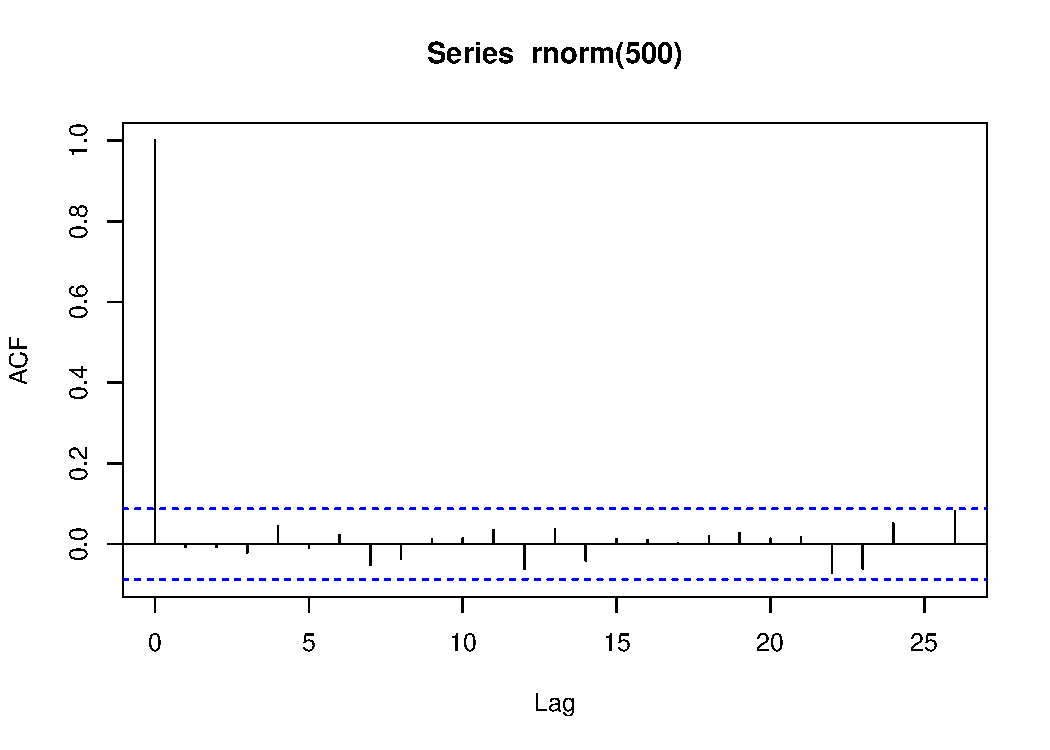
\includegraphics[width=0.75\textwidth]{acfwn130.pdf}
    \caption{ACF of white noise, sample length 130}\label{fig:acfwn130}
\end{figure}
\begin{minted}{R}
# Figure 2.1
acf(rnorm(500))
\end{minted}
In Figure~\ref{fig:acfwn130}:
{\color{blue}Let's then have a look at what the empirical autocorrelation
function looks like when we apply it to a strong white noise sample.
In this case, we are considering a strong Gaussian white noise
with variance 1. This is what the sample ACF looks like.
What we're plotting here is on the $ x $-axis we have the lags $ h $,
and on the $ y $-axis we have the magnitudes of the autocorrelation $ \hat{\rho}(h) $.
What we're seeing here
is $ \hat{\rho}(0)=1 $ (by definition). However, for lags other than zero,
for the other autocorrelations plotted, we can see that they are
relatively small compared to $ \hat{\rho}(0)=1 $,
which is the point of the blue lines (explained
in the next lecture). The basic interpretation of blue lines is that
if an autocorrelation would go inside the blue lines then you could imagine
that it would be consistent with the series being a strong white noise,
which is what we observe here. There's small violations that can occur by
sheer chance.}

\section{Modes of Convergence of Random Variables}
$ \hat{\gamma}(h) $ is an estimator of $ \gamma(h) $ when the data is stationary,
and we want to discuss the asymptotic properties of this estimator.

\underline{Introduce (Review)}
\begin{enumerate}
    \item Stochastic Boundedness (convergence of random variables): $ \mathcal{O}(p) $
          and $ \mathcal{o}(p) $
    \item Convergence in Probability
    \item Convergence in Distribution
\end{enumerate}
\begin{Definition}{Bounded in probability}{}
    Suppose $ \set{X_n}_{n\ge 1} $ is a sequence of random variables.
    We say that $ X_n $ is \textbf{bounded in probability}
    by $ Y_n $ if for all $ \varepsilon>0 $, there exists real numbers
    $ M,N $, so that for all $ n\ge N $,
    \[ \Prob*{\abs*{\frac{X_n}{Y_n}}> M}\le \varepsilon
    \]
    Notation: $ X_n=\mathcal{O}_p(Y_n) $, and in English, we say
    ``$ X_n $ is on the order of $ Y_n $.''
\end{Definition}
\begin{Definition}{Converges in probability}{}
    We say $ X_n $ \textbf{converges in probability}
    to $ X $ if for all $ \varepsilon>0 $,
    \[ \lim\limits_{{n} \to {\infty}} \Prob{\abs{X_n-X}>\varepsilon}=0 \]
    If $ a_n $ is a sequence of scalars, we abbreviate
    $ \displaystyle \frac{X_n}{a_n} $
    converges in probability to zero as
    \[ X_n=o_p(a_n)\iff \Prob*{\abs*{\frac{X_n}{a_n}}>\varepsilon}\to 0\text{ as }
        n\to\infty\quad (\forall\varepsilon>0) \]
    Hence, $ X_n $
    converges in probability to zero is denoted $ X_n=o_p(1) $.
    We also write $ X_n\stackrel{p}{\to}X $ to denote $ X_n $
    converges in probability to $ X $.
\end{Definition}
\begin{Definition}{Converges in distribution}{}
    We say that the sequence of scalar random variables
    $ X_n $ with respective CDF's $ F_n(x) $
    \textbf{converges in distribution} to $ X $ with CDF $ F(x) $
    if for all continuity points of $ y $ of $ F $,
    \[ \lim\limits_{{n} \to {\infty}} \abs{F_n(y)-F(y)}=0 \]
\end{Definition}
\begin{Remark}{}{}
    When $ F(x) $ is the CDF of a continuous random variable
    (e.g.\ a normal CDF), then
    \[ \lim\limits_{{n} \to {\infty}} \abs{F_n(y)-F(y)}=0\quad(\forall y\in\mathbf{R}) \]
\end{Remark}
\begin{Theorem}{Markov's Inequality}{markov}
    If $ \E{Y^2}<\infty $, then
    \[ \Prob{\abs{Y}\ge M}\le \frac{\E[\big]{Y^2}}{M^2}  \]
\end{Theorem}
\begin{Proof}{\Cref{thm:markov}}{}
    \begin{align*}
        \E{Y^2}
         & =\E{Y^2 I_{(\abs{Y}\ge M)}+Y^2 I_{(\abs{Y<M})}}                                    \\
         & =\E{Y^2 I_{(\abs{Y}\ge M)}} + \E{Y^2 I_{(\abs{Y<M})}}                              \\
         & \ge \E{Y^2 I_{(\abs{Y}\ge M)}}                                                     \\
         & \ge M^2\E{I_{(\abs{Y}\ge M)}}                         &  & \text{since }Y^2\ge M^2 \\
         & =M^2\Prob{\abs{Y}\ge M}
    \end{align*}
\end{Proof}
\begin{Remark}{Generalization of Markov's Inequality}{}
    If $ \E{Y^k}<\infty $, then
    \[ \Prob{\abs{Y}\ge M}\le  \frac{\E[\big]{\abs{Y}^k}}{M^k}  \]
\end{Remark}
\begin{Example}{}{}
    Suppose $ X_n $ is a strong white noise in $ L^2 $ ($ \E{X_0^2}<\infty $),
    and let
    \[ \bar{X}_T=\frac{1}{T} \sum_{t=1}^{T} X_t \]
    Then,
    \begin{enumerate}[(1)]
        \item $ \abs{\bar{X}_T}=o_p(1) $.
              \begin{align*}
                  \Var{\bar{X}_T}
                   & =\E{\bar{X}_T^2}                                                                                                             \\
                   & =\frac{1}{T^2} \E[\bigg]{\biggl(\sum_{t=1}^{T} X_t\biggr)^{\!2}}                                                             \\
                   & =\frac{1}{T^2} \sum_{t=1}^{T} \sum_{s=1}^{T}\Uunderbracket{\E{X_t X_s}}_{\ne 0\iff t=s}                                      \\
                   & =\frac{T}{T^2} \sum_{t=1}^{T} \E{X_t^2}                                                                                      \\
                   & =\frac{1}{T} \sum_{t=1}^{T} \E{X_0^2}                                                                                        \\
                   & =\frac{\sigma^2}{T}                                                                     &  & \text{since }\sigma^2=\E{X_0^2}
              \end{align*}
              Therefore, for $ \varepsilon>0 $, by Markov's Inequality we have
              \[ \Prob{\abs{\bar{X}_T}>\varepsilon}\le \frac{\E{\abs{\bar{X}_T}^2}}{\varepsilon^2}=
                  \frac{\sigma^2/T}{\varepsilon^2}\to 0\text{ as }T\to\infty  \]
              Hence, $ \abs{\bar{X}_T}\stackrel{p}{\to}0 $
        \item $ \bar{X}_T=\mathcal{O}_p(1/\sqrt{T}) $, as before
              \[ \Var*{\frac{\bar{X}_T}{1/\sqrt{T}}}=\Var{\sqrt{T}\bar{X}_T}=T\Var{\bar{X}_T}=\sigma^2 \]
              So by Markov's Inequality, for $ M>0 $
              \[ \Prob{\abs{\sqrt{T}\bar{X}_T}>M}\le \frac{\Var{\sqrt{T}\bar{X}_T}}{M^2}=\frac{\sigma^2}{M^2}
                  \to 0\text{ as }M\to\infty \]
              Hence $ \sqrt{T}\bar{X}_T=\mathcal{O}_p(1)\implies \bar{X}_T=\mathcal{O}_p(1/\sqrt{T}) $.
    \end{enumerate}
\end{Example}
\begin{Remark}{}{}
    Alternatively, we can show this using the CLT\@. By the CLT,
    \[ \sqrt{T}\bar{X}_T\stackrel{D}{\to}\N{0,\sigma^2} \]
    Therefore, if $ F_T\sim $ CDF of $ \sqrt{T}\bar{X}_T $ and $ \Phi\sim $
    CDF of $ \N{0,1} $ random variable we have
    \[ \abs*{F_T(x)-\Phi\biggl(\frac{x}{\sigma}\biggr)}\to 0\text{ as }T\to\infty\quad (\forall x\in\mathbf{R}) \]
    For $ \varepsilon>0 $, choose $ M $ such that
    \[ \Phi\biggl(-\frac{M}{\sigma}\biggr)=1-\biggl(\frac{M}{\sigma}\biggr)\le \frac{\varepsilon}{4} \]
    For this $ M $, choose $ T_0 $ such that if $ T\ge T_0 $, then
    \[ \abs*{F_T(-M)-\Phi\biggl(-\frac{M}{\sigma}\biggr)}\le \frac{\varepsilon}{4} \]
    and
    \[ \abs*{F_T(M)-\Phi\biggl(\frac{M}{\sigma}\biggr)}\le \frac{\varepsilon}{4} \]
    Then,
    \begin{align*}
        \Prob{\abs{\sqrt{T}\bar{X}_T}\ge M}
         & =F_T(-M)+(1-F_T(M))                                                                                                                                                            \\
         & =\Phi\biggl(-\frac{M}{\sigma}\biggr)+\biggl[1-\Phi\biggl(\frac{M}{\sigma} \biggr)\biggr]+F_T(-M)-\Phi\biggl(-\frac{M}{\sigma}\biggr)+\Phi\biggl(\frac{M}{\sigma}\biggr)-F_T(M) \\
         & \le \frac{\varepsilon}{4}+\frac{\varepsilon}{4} + \frac{\varepsilon}{4} + \frac{\varepsilon}{4}                                                                                \\
         & = \varepsilon
    \end{align*}
\end{Remark}
\begin{Remark}{}{}
    In general,
    \[ \frac{X_n}{a_n}\stackrel{D}{\to}\text{non-degenerate random variable}\implies X_n=\mathcal{O}_p(a_n)  \]
\end{Remark}
\begin{Remark}{Algebra of $ \mathcal{O}_p $ and $ o(p) $ notation}{}
    \begin{enumerate}
        \item If $ X_n=\mathcal{O}_p(a_n) $ and $ Y_n=\mathcal{O}_p(b_n) $, then
              \[ X_n+Y_n=\mathcal{O_p}(\max(a_n,b_n)) \]
        \item If $ X_n=o_p(1) $ and $ Y_n=o_p(1) $, then
              \[ X_n+Y_n=o_p(1) \]
        \item If $ X_n=o_p(1) $ and $ Y_n=o_p(1) $, then
              \[ X_n Y_n=o_p(1) \]
    \end{enumerate}
\end{Remark}
\begin{Example}{}{}
    Suppose $ W_t $ is a strong white noise
    in $ L^2 $ with $ \E{W_t^4}<\infty $. Let $ X_t=W_t+\theta W_{t-1} $
    for $ \theta\in\mathbf{R} $. Show that
    \[ \hat{\gamma}(1)\stackrel{p}{\to}\theta\sigma_W^2 \]
    \textbf{Solution.}
    \begin{align*}
        \bar{X}_T
         & =\frac{1}{T} \sum_{t=1}^{T} X_t                                                            \\
         & =\frac{1}{T} \sum_{t=1}^{T} (W_t+\theta W_{t-1})                                           \\
         & =\frac{1}{T} \sum_{t=1}^{T} W_t+\frac{\theta}{T} \sum_{t=}^{T} W_{t-1}                     \\
         & =o_p(1)                                                                &  & \text{by WLLN}
    \end{align*}
    \begin{align*}
        \hat{\gamma}(1)
         & =\frac{1}{T} \sum_{t=1}^{T-1} (X_t-\bar{X}_T)(X_{t+1}-\bar{X}_T)                                                                                           \\
         & =\frac{1}{T} \sum_{t=1}^{T-1} \bigl[X_t X_{t+1}-X_t\bar{X}_T-\bar{X}_T X_{t+1}+(\bar{X}_T)^2\bigr]                                                         \\
         & =\frac{1}{T} \sum_{t=1}^{T-1} X_t X_{t+1}-\frac{\bar{X}_T}{T}\sum_{t=1}^{T-1} X_t-\frac{\bar{X}_T}{T} \sum_{t=1}^{T-1} X_{t+1}+\frac{T-1}{T} (\bar{X}_T)^2 \\
         & =\frac{1}{T} \sum_{t=1}^{T-1} X_{t} X_{t+1}+R_{1}+ R_{2}+R_{3}
    \end{align*}
    Notice that $ R_{i}=o_p(1) $ for $ i=1,2,3 $ since, for example,
    $ \bar{X}_T=o_p(1) $ and $ \sum_{t=1}^{T} X_t=o_p(1) $ so their product is
    $ o_p(1) $; so we only need to focus on the first term.
    \begin{align*}
        \frac{1}{T} \sum_{t=1}^{T-1} X_t X_{t+1}
         & =\frac{1}{T} \sum_{t=1}^{T-1} (W_t+\theta W_{t-1})(W_{t+1}+\theta W_{t}) \\
         & =\frac{1}{T} \sum_{t=1}^{T-1}\theta W_{t}^2+G_{1}+G_{2}+G_{3}
    \end{align*}
    Now,
    \[ \frac{1}{T} \sum_{t=1}^{T-1} \theta W_{t}^2\stackrel{\text{a.s.}}{\to} \theta \E{W_t^2}=\theta\sigma_W^2 \]
    by strong law of large numbers. We now wish to calculate the variance of
    \[ G_{1}=\frac{1}{T} \sum_{t=1}^{T-1} W_{t} W_{t+1}. \]
    \[ \E{G_{1}}=\frac{1}{T} \sum_{t=1}^{T-1} \E{W_{t}W_{t+1}}=0 \]
    \begin{align*}
        \Var{G_{1}}
         & =\E{G_{1}^2}                                                                                                \\
         & =\frac{1}{T^2}\sum_{t=1}^{T-1} \sum_{s=1}^{T-1}\Uunderbracket{\E{W_{t}W_{t+1}W_{s}W_{s+1}}}_{\ne 0\iff s=t} \\
         & =\frac{T-1}{T^2} \sum_{t=1}^{T-1} \E{W_{t}^2W_{t+1}^2}=\frac{T-1}{T^2} \sigma_W^4\to 0\text{ as }T\to\infty
    \end{align*}
    By Markov's Inequality,
    \[ G_{1}=o_p(1) \]
    and similarly, for $ G_{2} $ and $ G_{3} $.
\end{Example}
\section{\texorpdfstring{$ \dagger $}{†} M-dependent CLT}
Suppose $ X_t $ is a mean zero strictly stationary time series
with $ \E{X_t^2}<\infty $. We are frequently faced
with the problems:
\begin{enumerate}[(1)]
    \item What is the approximate distribution of
          \[ \frac{1}{\sqrt{T}} \sum_{t=1}^{T} X_t=\sqrt{T}\bar{X}_T\stackrel{D}{\approx}\N{0,\sigma_X^2} \]
    \item If $ X_t $ is a strong white noise, what the approximate distribution of
          \[ \hat{\gamma}(h)=\frac{1}{T} \sum_{t=1}^{T-h}\Uunderbracket{X_t X_{t+h}}_{\text{not iid}}+o_p(1) \]
          $ X_t X_{t+h}=Y_{t} $ is strictly stationary.
\end{enumerate}
\begin{itemize}
    \item Only way to understand how $ \set{X_t}_{t\in\mathbf{Z}} $ behaves,
          we have to observe replicates of the process.
    \item If process is suitably ``weakly dependent,'' then we can observe
          replicates of the process by viewing in on overlapping windows.
\end{itemize}
\begin{Definition}{$ m $-dependent}{}
    We say a time series $ \set{X_t}_{t\in\mathbf{Z}} $ is $ m $\textbf{-dependent}
    for a positive integer $ m $, if for all
    \[ t_1<t_2<\cdots<t_{d_1}<s_1<s_2<\cdots<s_{d_2}\in\mathbf{Z} \]
    so that $ t_{d_1}+m\le s_1 $, then
    \[ (X_{t_1},\ldots,X_{t_{d_1}}) \]
    is \textbf{independent} of
    \[ (X_{s_1},\ldots,X_{s_{d_2}}) \]
\end{Definition}
\begin{Example}{}{}
    $ X_t=W_{t}+\theta W_{t-1} $ for $ \theta\in\mathbf{R} $
    and $ W_{t} $ is a strong white noise is $ 2 $-dependent.
\end{Example}
\begin{Theorem}{Generalization of the standard CLT to $ m $-dependent}{m_clt}
    Suppose $ X_t $ is a strictly stationary
    and $ m $-dependent time series for $ m\in\mathbf{Z}_{>0} $
    with $ \E{X_t}=0 $ and $ \E{X_t^2}<\infty $, then if
    \[ S_T=\frac{1}{\sqrt{T}} \sum_{t=1}^{T}X_t=\sqrt{T}\bar{X}_T
        \stackrel{D}{\to}\N{0,\sigma_m^2}\text{ as }T\to\infty  \]
    where
    \[ \sigma_m^2=\sum_{h=-m}^{m} \gamma(h)=\gamma(0)+2 \sum_{h=1}^{m} \gamma(h) \]
    Note that $ \sigma_m^2 $ is just the variance of $ S_T $
    and can be easily calculated.
\end{Theorem}
\begin{Definition}{Triangular array}{}
    We say $ \set{X_{i,j},1\le j\le n_i,1\le i<\infty} $ forms a
    \textbf{triangular array} of mean zero $ L^2 $ random
    variables, if $ \E{X_{i,j}}=0 $, $ \E{X_{i,j}^2}<\infty $, and
    for each $ i $-fixed we have $ X_{i,1},\ldots,X_{i,n_i} $
    are independent with $ n_i<n_i+1 $.
\end{Definition}
Visually, row-wise random variables are independent:
\[ \begin{matrix}
        X_{1,1} & \cdots & X_{1,n_1}             \\
        X_{2,1} & \cdots & \cdots    & X_{2,n_2} \\
        \vdots  & \ddots & \ddots    & \ddots
    \end{matrix} \]
\begin{Theorem}{Linderberg-Feller CLT for Triangular Arrays}{}
    Let $ \set{X_{i,j},1\le j\le n_i,1\le i<\infty} $
    be a triangular array of mean zero $ L^2 $ random variables.
    Define
    \[ \sigma_i^2=\sum_{j=1}^{n} \Var{X_{i,j}} \]
    and
    \[ S_i=\frac{1}{\sigma_i} \sum_{j=1}^{n_i} X_{i,j} \]
    If for $ \varepsilon>0 $,
    \[ \frac{1}{\sigma_i^2}\sum_{j=1}^{n_i} \E{X_{i,j}^2 I_{(\abs{X_{i,j}}>\varepsilon\sigma_i)}}\to 0
        \text{ as } i\to\infty \]
    then
    \[ S_i\stackrel{D}{\to}\N{0,1} \]
\end{Theorem}
\begin{Proof}{\Cref{thm:m_clt}}{pf_clt}
    Bernstein Blocking Argument: we take a given time series of length $ T $.

    Let $ a_T= $ big block size and $ m= $ little block size.
    We assume $ a_T\to\infty $ as $ T\to\infty $, but $ \displaystyle \frac{a_T}{T}\to 0 $.
    Then,
    \[ N=\text{number of blocks}=\biggl\lfloor \frac{T}{M+a_T} \biggr\rfloor \]
    \[ B_j=\set{i:(j-1)(a_T+m)+1\le i\le j a_T+(j-m)m} \]
    \[ b_j=\set{i:j a_T+(j-1)m+1\le i\le j(a_T+m)} \]
    Since $ a_T $ is increasing up to infinity, for $ T $
    sufficiently large, $ a_T>m $, and so
    by $ m $-dependence,
    \[ \sum_{t\in B_j}X_t  \]
    is independent of
    \[ \sum_{t\in B_k}X_t\quad(j\ne k)  \]
    similarly for $ B_j,B_k\to b_j,b_k $.
    \[ \frac{1}{\sqrt{T}}\sum_{t=1}^{T} X_t=\frac{1}{\sqrt{T}}
        \sum_{j=1}^{N}\sum_{t\in B_j}X_t+\frac{1}{\sqrt{T}} \sum_{j=1}^{N}
        \Uunderbracket{\sum_{t\in b_j}X_t}_{\text{iid}}+\text{Remainder}=G_1+G_2+G_3    \]
    We want to show the big blocks dominate.
    \[ \Var{G_2}=\frac{1}{T}
        \sum_{j=1}^{N}\E*{\biggl(\sum_{t\in b_j}X_t \biggr)^{\!2}}=
        \frac{N}{T}\E*{\biggl(\sum_{t=1}^{m} X_t\biggr)^{\!2}} \]
    Also,
    \[ \E*{\biggl(\sum_{t=1}^{m} X_t\biggr)^{\!2}}=\sum_{t=1}^{m} \sum_{s=1}^{m} \E{X_t X_s}=
        \sum_{t=1}^{m} \sum_{s=1}^{m}\gamma(\abs{t-s})  \]
    Let $ h=t-s $, set of possible values for $ h $ is $ m-\abs{h} $, so
    \[ =\sum_{h=1-m}^{m-1} (m-\abs{h})\gamma(h)<\infty \]
    noting that $ \gamma(h)=\gamma(-h) $, therefore for $ C $ as a constant, we have
    \[ \Var{G_2}=\frac{N}{T}
        C=\frac{\displaystyle \biggl\lfloor \frac{T}{a_T+m} \biggr\rfloor}{T}(C)\to 0\text{ as }a_T\to\infty  \]
    and hence $ G_2=o_p(1) $.

    Let's deal with the big block terms. Notice
    \[ G_1=\frac{1}{\sqrt{T}}=\sum_{j=1}^{N} \sum_{t\in B_j}X_t=
        \sum_{j=1}^{N}\frac{\sum_{t\in B_j} X_t}{\sqrt{T}}=\sum_{j=1}^{N}Y_j  \]
    where $ Y_{j} $ is a triangular array. So,
    $ \Var{G_1}=\sum_{j=1}^{N} \Var{Y_j} $.
    \begin{align*}
        \Var{Y_j}
         & =\Var{Y_1}                                                 \\
         & =\frac{1}{T} \E*{\biggl(\sum_{t=1}^{a_T}X_t\biggr)^{\!2}}  \\
         & =\frac{1}{T}\sum_{t=1}^{a_T} \sum_{s=1}^{a_T} \E{X_t X_s}  \\
         & =\frac{1}{T} \sum_{h=1-a_T}^{a_T-1} (a_T-\abs{h})\gamma(h)
    \end{align*}
    Note that since the process is $ m $-dependent, $ \gamma(h)=0 $ if $ \abs{h}\ge m $.
    Continuing,
    \[ \frac{1}{T} \sum_{h=1-a_T}^{a_T-1} (a_T-\abs{h})\gamma(h)=
        \sum_{h=-m}^{m} (a_T-\abs{h})\gamma(h) \]
    Therefore,
    \[ \Var{G_1}=\Uunderbracket{\frac{N}{T}}_{\approx 1/a_T}
        \sum_{h=-m}^{m}(a_T-\abs{h})\gamma(h) \to \sum_{h=-m}^{m} \gamma(h)\text{ as }T\to\infty \]
    Therefore, the variance of $ G_1 $ is bounded.
    We showed $ \sigma_N^2=\Var{G_1}\approx $ constant. So, we must show
    \[
        \sum_{j=1}^{N} \E{\Uunderbracket{Y_{j}^2}_{\text{iid}} I_{(\abs{Y_{j}}>\varepsilon\sigma_N)}}=
        N\E{Y_{1}^2 I_{(\abs{Y_{1}}>\varepsilon\sigma_N)}} \to 0\text{ as } T\to\infty
    \]
    \emph{Aside}:
    \begin{align*}
        \E[\big]{\abs{Y}^{2+\delta}}
         & \ge \E[\big]{\abs{Y}^{2+\delta}I_{(\abs{Y}>\varepsilon)}}           \\
         & \ge \varepsilon^\delta\E[\big]{\abs{Y}^2 I_{(\abs{Y}>\varepsilon)}} \\
    \end{align*}
    \[ \implies \E[\big]{\abs{Y}^2 I_{(\abs{Y}>\varepsilon)}}\le \frac{\E[\big]{\abs{Y}^{2+\delta}}}{\varepsilon^\delta} \]
    It may be shown that for $ C>0 $
    \[ \E[\big]{\abs{Y_j}^{2+\delta}}\le C\biggl(\frac{a_T}{T} \biggr)^{\frac{2+\delta}{2}} \]
    So
    \begin{align*}
        N\E{Y_{1}^2 I_{(\abs{Y_{1}}>\varepsilon\sigma_N)}}
         & \le \frac{N}{(\varepsilon\sigma_N)^\delta}C\biggl(\frac{a_T}{T} \biggr)^{\frac{2+\delta}{2}} \\
         & =\frac{C}{(\varepsilon\sigma_N)^\delta}
        \frac{N a_T}{T}\biggl(\frac{a_T}{T} \biggr)^{\delta/2}\to 0\text{ as }T\to\infty
    \end{align*}
    Therefore, by~\Cref{thm:m_clt}
    \[ \frac{G_1}{\sigma_N}\stackrel{D}{\to}\N{0,1}\text{ as }T\to\infty  \]
    and since
    \[ \sigma_N^2\to \sum_{j=-m}^{m} \gamma(j) \]
    we have
    \[ G_1\stackrel{D}{\to}\N*{0,\sum_{h=-m}^{m} \gamma(h)} \]
    Since $ G_2=o_p(1) $ we have
    \[ \frac{1}{\sqrt{T}}\sum_{t=1}^{T} X_t\stackrel{D}{\to}\N*{0,\sum_{h=-m}^{n} \gamma(h)}  \]
\end{Proof}
\section{\texorpdfstring{$ \dagger $}{†} Two Plus Delta Moment Calculation}
We want to show
\[ \E{\abs{Y_1}^{2+\delta}}\le C\biggl(\frac{a_T}{T} \biggr)^{\frac{2+\delta}{2}} \]
where
\[ Y_1=\frac{1}{\sqrt{T}} \sum_{t=1}^{a_T} X_t \]
$ a_T= $ big block size $ \to\infty $ as $ T\to\infty $
\[ \frac{a_T}{T} \to 0 \]
$ X_t $ are $ m $-dependent random variables.
\[ \E{\abs{X_i}^{2+\delta}}<\infty\quad(\delta>0)\iff
    \E*{\abs[\bigg]{\sum_{t=1}^{a_T} X_t}^{2+\delta}}\le C a_T^{\frac{2+\delta}{2}} \]
\begin{Theorem}{Rosenthal's Inequality}{rosenthal_ineq}
    If $ X_1,\ldots,X_n $ are independent random variables
    with $ \E{\abs{X_i}^{2+\delta}}<\infty $ for $ \delta>0 $, then
    \[ \E*{\abs[\bigg]{\sum_{i=1}^{n} X_i}^{2+\delta}}<c_p n^{\delta/2}\sum_{i=1}^{n}
        \E[\big]{\abs{X_i}^{2+\delta}} \]
    In particular, if $ X_1,\ldots,X_n $ are i.i.d., then
    \[ \E{\abs[\bigg]{\sum_{i=1}^{n} X_i}^{2+\delta}}\le c_p n^{\frac{2+\delta}{2}}
        \E[\big]{\abs{X_1}^{2+\delta}} \]
\end{Theorem}
\begin{Proof}{\Cref{thm:rosenthal_ineq}}{}
    See Petrov, Limit theorems of Probability Theory, p.g.\ 59.
\end{Proof}
\begin{Proposition}{}{prop1}
    For arbitrary random variables $ X_1,\ldots,X_n $,
    \[ \E*{\abs[\bigg]{\sum_{i=1}^{n} X_i}^{2+\delta}}\le n^{(2+\delta)-1}
        \sum_{i=1}^{n}\E[\big]{\abs{X_i}^{2+\delta}} \]
\end{Proposition}
\begin{Proof}{\Cref{prop:prop1}}{}
    By Jensen's Inequality, for $ a_1,\ldots,a_n\in\mathbf{R} $,
    \[ \abs[\bigg]{\frac{1}{n} \sum_{i=1}^{n} a_i}^{2+\delta}\le \frac{1}{n} \sum_{i=1}^{n} \abs{a_i}^{2+\delta} \]
    Since $ f(x)=x^{2+\delta} $ is convex, rearranging yields
    \[ \abs[\bigg]{\sum_{i=1}^{n} a_i}^{2+\delta}\le
        n^{(2+\delta-1)}\sum_{i=1}^{n} \abs{a_i}^{2+\delta} \]
    Replace $ a_i\sim X_i $, take expectation.
\end{Proof}
\[ \sum_{t=1}^{a_T} X_t=\sum_{j=0}^{m}
    \sum_{\substack{t=j\mod (m+1)\\1\le t\le a_T}}X_t  \]
Variables in the second sum are separated by at least
$ m $-time steps, and hence i.i.d.\ Therefore,
\begin{align*}
    \E{\abs[\bigg]{\sum_{t=1}^{a_T} X_t}^{2+\delta}}
     & \le (m=1)^{(2+\delta)-1}
    \E[\bigg]{\abs[\bigg]{\sum_{\substack{t=j\mod (m+1)                                                                                                    \\1\le t\le a_T}}X_t}^{2+\delta}} & \quad & \text{by~\Cref{prop:prop1}}\\
     & \le (m+1)^{(2+\delta)-1}\biggl(\frac{a_T}{m+1} \biggr)^{\frac{2+\delta}{2} }\E[\big]{\abs{X_1}^{2+\delta}} &  & \text{by~\Cref{thm:rosenthal_ineq}} \\
     & =C a_T^{\frac{2+\delta}{2}}
\end{align*}
where $ C $ is the same constant as in the proof of~\Cref{thm:m_clt}.

\section{\texorpdfstring{$ \dagger $}{†} Linear Process CLT}
\begin{Example}{}{}
    $ \displaystyle X_t=\sum_{\ell=0}^{m} \psi_\ell W_{t-\ell} $
    where $ \set{W_t}_{t\in\mathbf{Z}} $ is
    is a strong white noise in $ L^2 $.

    A general linear process $ \displaystyle X_t=\sum_{\ell=0}^{m} \psi_\ell W_{t-\ell} $
    is \underline{not} $ m $-dependent.
\end{Example}
\begin{Theorem}{Basic Approximation Theorem (BAT)}{bat}
    Suppose $ X_n $ is a sequence of random variables
    so that there exists an array
    \[ \set{Y_{n,m},m,n\ge 1} \]
    so that:
    \begin{enumerate}[(1)]
        \item For each fixed $ m $, $ Y_{m,n}\stackrel{D}{\to}Y_m $
              as $ n\to\infty $.
        \item $ Y_m\stackrel{D}{\to} Y $ as $ m\to\infty $ for some random variable $ Y $.
        \item For all $ \varepsilon>0 $,
              \[ \lim\limits_{{m} \to {\infty}}
                  \Bigl[\lim\sup\limits_{{n} \to {\infty}}
                  \Prob{\abs{X_n-Y_{n,m}>\varepsilon}} \Bigr]=0 \]
    \end{enumerate}
    Then $ X_n\stackrel{D}{\to}Y $ as $ n\to\infty $.
\end{Theorem}
\begin{Remark}{}{}
    $ Y_{m,n} $ is often an ``$ m $-dependent'' approximation to $ X_n $
\end{Remark}
\begin{Proof}{\Cref{thm:bat}}{}
    Shumway and Stoffer using characteristic functions.
\end{Proof}
\begin{Theorem}{Linear Process CLT}{lin_clt}
    Suppose $ X_t=\sum_{\ell=0}^{\infty} \psi_\ell W_{t-\ell} $ is a causal
    linear process with $ \sum_{\ell=0}^{\infty} \abs{\psi_\ell}<\infty $
    with $ \set{W_t}_{t\in\mathbf{Z}} $ is a strong white noise in
    $ L^2 $. If
    \[ S_t=\frac{1}{\sqrt{T}} \sum_{t=1}^{T} X_t \]
    then
    \[ S_T\stackrel{D}{\to}\N*{0,\sum_{\ell=-\infty}^{\infty} \gamma(\ell)}\text{ as }
        T\to\infty \]
\end{Theorem}
\begin{Proof}{\Cref{thm:lin_clt}}{}
    $ X_t $ is strictly (and weakly) stationary.
    \begin{align*}
        \gamma(h)
         & =\E{X_t X_{t+h}}                                                                                                                                          \\
         & =\E[\bigg]{\biggl(\sum_{\ell=0}^{\infty} \psi_\ell W_{t-\ell}\biggr)\biggl(\sum_{j=0}^{\infty} \psi_j W_{t+h-j}\biggr)}                                   \\
         & =\sum_{\ell=0}^{\infty}\sum_{j=0}^{\infty} \psi_\ell\psi_j\E{W_{t-\ell}W_{t+h-j}}                                       & \quad & \text{Fubini's Theorem} \\
         & = \sum_{\ell=0}^{\infty} \psi_\ell \psi_{\ell+h}\sigma_W^2
    \end{align*}
    Then,
    \[ \sum_{h=-\infty}^{\infty} \gamma(h)=\sum_{h=-\infty}^{\infty}
        \abs[\bigg]{\sum_{\ell=0}^{\infty} \psi_\ell \psi_{\ell+h}\sigma_W^2}
        \le \sum_{\ell=0}^{\infty} \abs{\psi_\ell}\sum_{h=-\infty}^{\infty} \abs{\psi_h}\sigma_W^2<\infty \]
    So $ \sum_{h=-\infty}^{\infty} \gamma(h) $ is well-defined.
    Note that $ \E{S_T}=0 $ since $ \E{X_t}=0 $. Also,
    \[ \Var{S_T}=\frac{1}{T} \sum_{t=1}^{T} \sum_{s=1}^{T} \E{X_tX_s}=
        \frac{1}{T} \sum_{h=1-T}^{T-1} (T-\abs{h})\gamma(h)=\sum_{h=1-T}^{T-1}
        \biggl(1-\frac{\abs{h}}{T} \biggr)\gamma(h) \]
    Note that $ \displaystyle \biggl(1-\frac{\abs{h}}{T} \biggr)\le \abs{\gamma(h)} $
    since $ \set{\abs{\gamma(h)}} $ is summable by Dominated Convergence Theorem (DCT).

    Define
    \[ X_{t,m}=\sum_{\ell=0}^{m} \psi_\ell W_{t-\ell} \]
    \[ S_{T,m}=\frac{1}{\sqrt{T}} \sum_{t=1}^{T} X_{t,m} \]
    is a $ m $-dependent approximation to $ S_T $.
    \begin{enumerate}[(1)]
        \item By the $ m $-dependent CLT,
              \[ S_{T,m}\stackrel{D}{\to}\N*{0,\sum_{h=-m}^{m} \gamma_m(h)}\coloneq
                  S_m^\prime \]
              and $ \gamma_m(h)=\E{X_{t,m}X_{t+h,m}} $.
        \item By DCT,
              \[ \sum_{h=-m}^{m} \gamma_m(h)
                  \stackrel{m\to\infty}{\to}\sum_{h=-\infty}^{\infty} \gamma(h) \]
              and hence
              \[ S_m^\prime\stackrel{D}{\to}\N*{0,\sum_{h=-\infty}^{\infty} \gamma(h)} \]
        \item \begin{align*}
                  \E{(S_{T,m}-S_T)^2}
                   & =\frac{1}{T} \E*{\biggl(\sum_{t=1}^{T}(X_t-X_{t,m}) \biggr)^{\!2}} \\
                   & \le \sum_{h=1-T}^{T-1} \biggl(1-\frac{\abs{h}}{T} \biggr)
                  \sum_{\ell=m+1}^{\infty}\abs{\psi_\ell}\abs{\psi_{\ell+h}}\sigma_W^2  \\
                   & \le \sum_{\ell=m+1}^{\infty} \abs{\psi_\ell}
                  \biggl(\sum_{h=-\infty}^{\infty} \abs{\psi_h}\biggr)\sigma_W^2\to 0\text{ as }m\to\infty
              \end{align*}
    \end{enumerate}
    So condition (3) of the BAT is satisfied using Markov's Inequality. Therefore,
    \[ S_t=\frac{1}{\sqrt{T}}\sum_{t=1}^{T} X_t\stackrel{D}{\to}\N*{0,\sum_{h=-\infty}^{\infty} \gamma(h)}  \]
\end{Proof}
\section{Asymptotic Properties of Empirical ACF}
If $ X_1,\ldots,X_T $ is an observed time series
which we think was generated by a stationary process, then
$ \Cov{X_t,X_{t+h}} $ does not depend on $ t $. Recall that
\[ \hat{\gamma}(h)=\frac{1}{T} \sum_{t=1}^{T-h}(X_t-\bar{X})(X_{t+h}-\bar{X}) \]
\[ \rho(h)=\Corr{X_t,X_{t+h}}=\frac{\gamma(h)}{\gamma(0)} \]
\[ \hat{\rho}(h)=\frac{\hat{\gamma}(h)}{\hat{\gamma}(0)}  \]
Questions:
\begin{enumerate}[(1)]
    \item Are $ \hat{\gamma} $ and $ \hat{\rho} $ consistent?
    \item What is the approximate distribution of $ \hat{\gamma}(h) $
          and $ \hat{\rho}(h) $.
\end{enumerate}
\textbf{Consistency}: By adding and subtracting $ \mu $ in the definition
of $ \hat{\gamma}(h) $, we may assume WLOG that $ \E{X_t}=0 $.

Suppose $ \set{X_t}_{t\in\mathbf{Z}} $ is strictly stationary, and
\[ X_t=g(W_t,W_{t-1},\ldots) \]
We first need to establish the consistency of
\[ \bar{X}=\frac{1}{T} \sum_{t=1}^{T} X_t \]
where $ X_t $'s are not i.i.d.\ so Law of Large numbers
does not work. Instead, we would use the Ergodic Theorem, but
we will not cover it here. Therefore,
\[ \bar{X}\stackrel{P}{\to}0 \]
Furthermore,
\begin{align*}
    \hat{\gamma}(h)
     & =\frac{1}{T} \sum_{t=1}^{T-h} (X_t-\bar{X})(X_{t+h}-\bar{X}) \\
     & =\frac{1}{T} \sum_{t=1}^{T-h} X_t X_{t+h}-
    \bar{X}\frac{1}{T} \sum_{t=1}^{T-h} X_t -\bar{X}\frac{1}{T} \sum_{t=1}^{T-h} X_{t+h}+
    \frac{T-h}{T} (\bar{X})^2
\end{align*}
where we note that the last three terms converge in probability to 0 by the Ergodic Theorem.

Also, note that $ \E{X_t X_{t+h}}=\gamma(h) $ and
\[ X_{t}X_{t+h}=g_h(W_{t+h},W_{t+h-1},\ldots) \]
Again, by the Ergodic Theorem,
\[ \frac{1}{T} \sum_{t=1}^{T-h} X_t X_{t+h}\stackrel{P}{\to}\gamma(h) \]
Therefore, $ \hat{\gamma}(h)\stackrel{P}{\to}\gamma(h) $
and $ \displaystyle \hat{\rho}(h)=\frac{\hat{\gamma}(h)}{\hat{\gamma}(0)}\stackrel{P}{\to}\rho(h) $
under strict stationarity and $ \E{X_t^2}<\infty $.

\textbf{Distribution of} $ \hat{\gamma}(h) $: Consider
simple (but most important case) when $ \set{X_t}_{t\in\mathbf{Z}} $
is a strong white noise with $ \E{X_t^4}<\infty $. The finite
4th moment assumption is not really assumed here, but this will
be explained why it's classically assumed.
\[ \hat{\gamma}(h)\stackrel{P}{\to}0 \]
Similarly,
\[ \hat{\gamma}(h)=\Uunderbracket{\frac{1}{T}\sum_{t=1}^{T-h}X_t X_{t+h}}_{\tilde{\gamma}(h)}+R   \]
Note that $ \E{\tilde{\gamma}(h)}=0 $ for $ h\ge 1 $. Also,
\[ \Var{\tilde{\gamma}(h)}=\E{\tilde{\gamma}^2(h)}=
    \frac{1}{T^2}\sum_{t=1}^{T-h} \sum_{s=1}^{T-h}
    \E{X_t X_{t+h}X_s X_{s+h}} \]
is non-zero only when $ t=s $, so
\[ \Var{\tilde{\gamma}(h)}=\frac{1}{T^2} \sum_{t=1}^{T-h} \E{X_t^2 X_{t+h}^2}=
    \frac{T-h}{T^2} \sigma_X^4 \]
where $ \E{X_t^2}=\sigma_X^2 $. Therefore,
\[ \Var{\sqrt{T}\tilde{\gamma}(h)}
    \stackrel{T\to\infty}{\to}\sigma_X^4 \]
\begin{Theorem}{}{sigma4}
    If $ \set{X_t}_{t\in\mathbf{Z}} $ is a strong white noise
    with $ \E{X_t^4}<\infty $, then
    \[ \sqrt{T}\tilde{\gamma}(h)=\frac{1}{\sqrt{T}} \sum_{t=1}^{T-h} X_t X_{t+h}
        \stackrel{D}{\to}\N{0,\sigma_X^4} \]
\end{Theorem}
\begin{Proof}{\Cref{thm:sigma4}}{}
    Using Martingale CLT which is derived from $ m $-dependent CLT.\@
\end{Proof}
\begin{Corollary}{}{}
    It follows that if
    \[ \sqrt{T}\hat{\gamma}\stackrel{D}{\to}\N{0,\sigma_X^4} \]
    and $ \hat{\gamma}(0)\stackrel{P}{\to}\sigma_X^2 $ (SLLN), then by Slutsky's Theorem,
    \[ \sqrt{T}\frac{\hat{\gamma}(h)}{\hat{\gamma}(0)}=
        \sqrt{T}\hat{\rho}(h)\stackrel{D}{\to}\N{0,1}  \]
\end{Corollary}
If $ \set{X_t}_{t\in\mathbf{Z}} $ is a strong white noise,
\[ \biggl(-\frac{z_{\alpha/2}}{\sqrt{T}} ,\frac{z_{\alpha/2}}{\sqrt{T}} \biggr) \]
is a $ (1-\alpha) $ prediction interval for $ \hat{\rho}(h) $
for all $ h $ with $ T $ large where $ \Phi(z_{\alpha/2})=1-\alpha $. Hence,
\[ \biggl(\frac{-1.96}{\sqrt{T}},\frac{1.96}{\sqrt{T}} \biggr) \]
is an approximate $ 95\% $ prediction interval for $ \hat{\rho}(h) $
assuming the data is generated by a strong white noise process.

Now, we know that the blue boundaries are $ \displaystyle \pm \frac{1.96}{\sqrt{T}} $
in~\Cref{fig:acfwn130}. Also, we might be able to say that
exists mild serial correlation at lag 1 of the ACF for Figure 2.2.
